\documentclass{article}
\usepackage{graphicx}
\graphicspath{{Imagenes/}}

%\font\titleFont = cmr12 at 40pt
%\title{{\titleFont Trabajo Pr\'actico de Probabilidad y Estad\'istica}}
%\title{{\fontsize{30cm}{1cm}\selectfont Trabajo Pr\'actico de Probabilidad y Estad\'istica}}
\title{{\Huge Trabajo Pr\'actico de Probabilidad y Estad\'istica:
	\linebreak 
	Ley de los Grandes N\'umeros y el Teorema Central del L\'imite}}
\author{Buceta Diego, Springhart Gonzalo, Tasat Dylan}

\begin{document}
	\maketitle %Ponemos el título
	\thispagestyle{empty} %Sacamos el número de pie de página
	
	\newpage %Saltamos a la próxima página
	\setcounter{page}{1} %Reseteamos el contador
	
	%Ahora empieza el documento de verdad
	
	\section{Pre\'ambulo}
	La Ley de los Grandes N\'umeros y el Teorema Central del L\'imite son temas fundamentales de la probabilidad y la estad\'istica, sin embargo entender ambos no es trivial. Mediante este trabajo buscamos entender los conceptos de la Ley de los Grandes N\'umeros y el Teorema Central del L\'imite mediante ejercicios que ponen en evidencia el cumplimiento de ambos.
	
	\newpage
	
	\section{Primer Ejercicio}
	En este ejercicio, trabajamos con una variable aleatoria exponencial de par\'ametro $\lambda = \frac{1}{4}$. Con esta variable generamos 3000 experimentos de $n$ observaciones cada uno, es decir el primer experimento tiene una observaci\'on, el segundo dos y as\'i sucesivamente. 
	\linebreak
Si tomamos la media de cada uno de los experimentos y la graficamos podermos ver que queda el siguiente gr\'afico

	
%	\begin{figure}
%		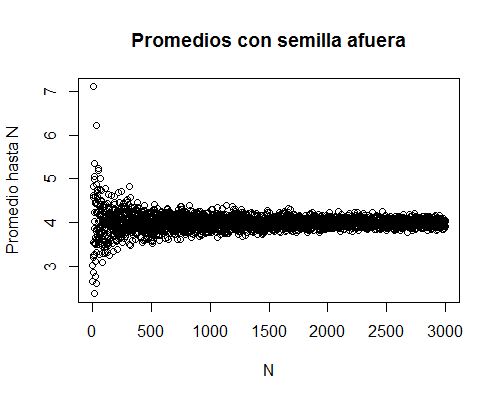
\includegraphics[scale=0.4]{grafico1}
%		\centering
%	\end{figure}

	{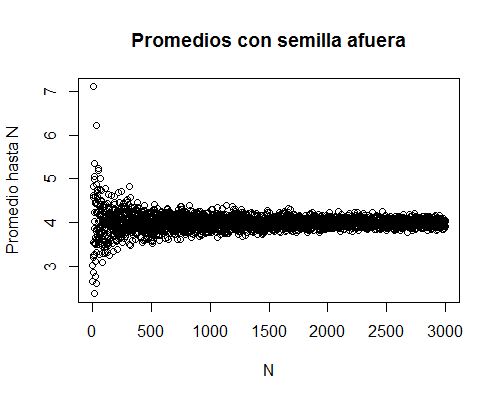
\includegraphics[scale=0.75]{grafico1}
	\centering}
	
	Se puede observar que el gr\'afico tiene una pinta similar al de una normal, esto nos sirve para ver una representaci\'on del Teorema Central del L\'imite, que dice que si se tienen $X_1,...,X_n$ variables aleatorias i.i.d. con esperanza $\mu$ y varianza $\sigma^2$ entonces si $n$ es lo suficientemente grande, la variable aleatoria $\bar{X} = \frac{1}{n}\sum_{i=1}^{n} X_i$ tiene aproximadamente una distribuci\'on $\mathcal{N}(\mu, \frac{\sigma^2}{n})$.
	\linebreak
	\linebreak
	\begin{flushleft}
		{\large Diferencias de Gr\'aficos}
		\linebreak
	\end{flushleft}
	Como el t\'itulo ind\'ica, el gr\'afico anterior fu\'e computado en R seteando primero una semilla afuera de un ciclo for. Si a esa semilla la colocamos dentro del ciclo el gr\'afico mostrado cambia al siguiente
	
	
	{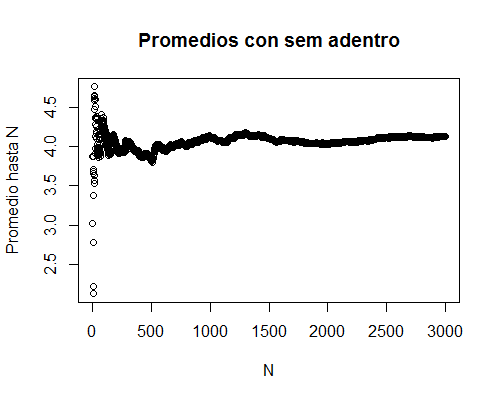
\includegraphics[scale=0.75]{grafico2}
	\centering}
	
	Como se puede ver, los dos gr\'aficos son diferentes, \textquestiondown A qu\'e se debe \'esta diferencia? Se debe al modo en que R trabaja con las semillas al momento de generar datos al azar.
	
	En R al pedir que se genere un valor al azar, la \'unica forma de que ese valor siempre sea el mismo es setear la semilla antes de generarlo. Si se pide que se generen m\'as observaciones de las que se generaron antes, la \'unica observaci\'on distinta va a ser la final, es decir, si primero genero una variable con $n$ observaciones y despu\'es genero una nueva variable con $n+1$ observaciones, las primeras $n$ observaciones de esa nueva variable van a ser iguales a las $n$ de la anterior si seteo la misma semilla antes de generarla.
	En el segundo gr\'afico se grafican las medias calculadas de la misma forma que en el primer gr\'afico, pero en este caso, como la semilla esta dentro del ciclo for, las observaciones de cada experimento son las mismas, la \'unica diferencia es la cantidad de observaciones que tiene cada experimento.
	En este segundo gr\'afico tambi\'en se puede ver como las medias se empiezan a aproximar a la esperanza de la variable aleatoria exponencial cuando $n$ es grande.
	\newpage
	
	\section{Segundo Ejercicio}
	
	\newpage
	
	\section{Tercer Ejercicio}
	
	\newpage
	
	\section{Cuarto Ejercicio}
	
	\newpage
	
	\section{Conclusiones}
	
	\newpage
	
\end{document}
